\documentclass[border=4pt]{standalone}
\usepackage{amsmath,amssymb,tikz}\usetikzlibrary{arrows.meta,calc}
\definecolor{figB}{RGB}{31,90,166}\definecolor{figR}{RGB}{176,48,48}\definecolor{figG}{RGB}{46,125,50}\definecolor{figO}{RGB}{214,120,20}
\begin{document}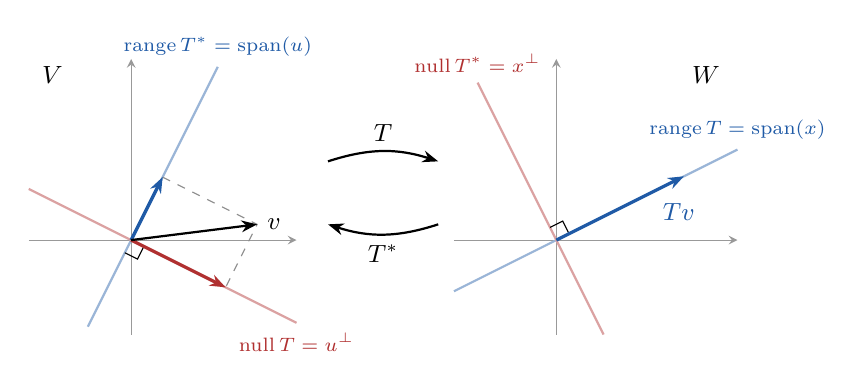
\begin{tikzpicture}[scale=1.0,>={Stealth[length=2mm]}]
% ---- V: u = (1,2) direction, v = (1.6,0.2) = (0.4,0.8) + (1.2,-0.6)
\begin{scope}
\draw[black!40,thin,-stealth] (-1.3,0)--(2.1,0); \draw[black!40,thin,-stealth] (0,-1.2)--(0,2.3);
\draw[thick,figB!45] (-0.55,-1.1)--(1.1,2.2) node[above,font=\scriptsize,figB]{$\operatorname{range}T^*=\operatorname{span}(u)$};
\draw[thick,figR!45] (-1.3,0.65)--(2.1,-1.05) node[below,font=\scriptsize,figR]{$\operatorname{null}T=u^\perp$};
\draw[thin] ($(0,0)!0.18cm!(-1,-2)$) coordinate(a) -- ($(a)!0.18cm!-90:(0,0)$) coordinate(b) -- ($(0,0)!0.18cm!(2,-1)$);
\draw[dashed,black!45] (0.4,0.8)--(1.6,0.2)--(1.2,-0.6);
\draw[->,very thick,figB] (0,0)--(0.4,0.8);
\draw[->,very thick,figR] (0,0)--(1.2,-0.6);
\draw[->,thick] (0,0)--(1.6,0.2) node[right,font=\small]{$v$};
\node[font=\small] at (-1.0,2.1) {$V$};
\end{scope}
\draw[->,thick] (2.5,1.0) to[bend left=18] node[above,font=\small]{$T$} (3.9,1.0);
\draw[<-,thick] (2.5,0.2) to[bend right=18] node[below,font=\small]{$T^*$} (3.9,0.2);
% ---- W: x = (2,1) direction, Tv = <v,u> x = (1.62,0.81)
\begin{scope}[xshift=5.4cm]
\draw[black!40,thin,-stealth] (-1.3,0)--(2.3,0); \draw[black!40,thin,-stealth] (0,-1.2)--(0,2.3);
\draw[thick,figB!45] (-1.3,-0.65)--(2.3,1.15) node[above,font=\scriptsize,figB]{$\operatorname{range}T=\operatorname{span}(x)$};
\draw[thick,figR!45] (0.6,-1.2)--(-1.0,2.0) node[above,font=\scriptsize,figR]{$\operatorname{null}T^*=x^\perp$};
\draw[thin] ($(0,0)!0.18cm!(2,1)$) coordinate(a) -- ($(a)!0.18cm!-90:(0,0)$) coordinate(b) -- ($(0,0)!0.18cm!(-1,2)$);
\draw[->,very thick,figB] (0,0)--(1.62,0.81) node[pos=0.75,below right,font=\small,figB]{$Tv$};
\node[font=\small] at (1.9,2.1) {$W$};
\end{scope}
\end{tikzpicture}\end{document}
